Although we formally described the \textit{query split} in Section \ref{S3}, there are still some relatively flexible components. In this section, we examine these components in more detail, and provide some concrete implementations: the query splitting algorithm (in Section \ref{S41}) and the criterion for selecting which sub-query to execute each time (in Section \ref{S42}). However, since our paper aims to verify the general effectiveness of \textit{query split}, an in-depth research of these components is beyond the scope of this paper. The contents of this section only serve as some preliminary designs for reference.
\subsection{Query Splitting Algorithm} \label{S41}
\textcolor{blue}{
    In this section, we propose our query splitting algorithm \textit{RelationshipCenter}, and two other algorithms (\textit{MinSubquery} and \textit{EntityCenter}) for later experimental contrast.
}
    \subsubsection{RelationshipCenter} \label{S412}
        Because \textit{query split} needs to materialize the result of sub-queries, it would be beneficial to attempt to constrain the size of sub-query results when constructing the sub-queries. There are several potential benefits for doing this: first, a small sub-query result can speed up the later execution, as the completed sub-queries will often be used in other sub-queries. Another benefit is that it improves the framework's robustness by using less memory. In \textit{query split}, each sub-query result must be materialized in memory after execution, and hence sub-queries with bounded result sizes lead to more stable memory usage.\par
\textcolor{blue}{
        According to Axel et al. \cite{USE}, if all the operators in a query are non-expanding operators, the result size of the query is constrained. The non-expanding operator is a kind of operator whose result size does not exceed the input size. For example, primary-foreign-key join ensures the join result will not exceed the relation that contains the foreign key. Besides, filter operation also belongs to the non-expanding operator. According to the property of non-expanding operators, we can constrain the result size of sub-queries. Suppose each join in a sub-query is the primary-foreign-key join and all foreign keys locate in the same relation. In that case, the size of the sub-query result will not exceed the size of that relation.
}\par
        To ensure the above conditions, we first introduce two new concepts: entity relation and relationship relation, which are inspired by the entity-relationship diagram \cite{paper32}. If the primary key of a relation is referenced by another relation as foreign key, we denote such relation as an entity relation. For relations that do not have a primary key or their primary keys are not referenced by any other relation, we denote them as relationship relations.\par
\textcolor{blue}{
        With the above definitions, we can see that when a sub-query consists of a relationship relation with several entity relations, each join in this sub-query is the primary-foreign-key join, and thus the cardinality of the sub-query result will not exceed the size of the relationship relation. Based on this, we propose the \textit{RelationshipCenter} algorithm to control the size of each sub-query. The algorithm ensures that most sub-queries contain one relationship and multiple entity relations. The concrete steps of \textit{RelationshipCenter} are shown as follows.
}
        \begin{itemize}[leftmargin = 15pt]
            \item First, we classify all relations into two types: relationship and entity by the above definitions.
            \item Next, we remove redundant select predicates, and we prefer to reserve foreign-key joins as much as possible.
            \item Then, we construct a directed graph for the given query, in which each vertex represents a relation. For each foreign-key join predicate, we create an edge from the relation which contains the foreign key to the relation where primary key comes. For every other select predicate that spans multiple relations, we consider all possible pairs from the involved relations, and create one or two edges between them, depending on their relation types: if both relations are the same type, we create two edges in both directions. Otherwise, we create an edge from relationship relation to entity relation.
            \item Last, for each relation that connects to other relations, we create a sub-query based on this relation. The relation set of the sub-query contains the given relation and all relations it links to. The select predicate set contains all predicates over the relation set.
        \end{itemize}\par
        Example \ref{E4} demonstrates how \textit{RelationshipCenter} works.
        \begin{figure}[htb]
            \subfigure[\normalsize{Global query}]
            {
                \begin{minipage}[t]{0.47\linewidth}
                    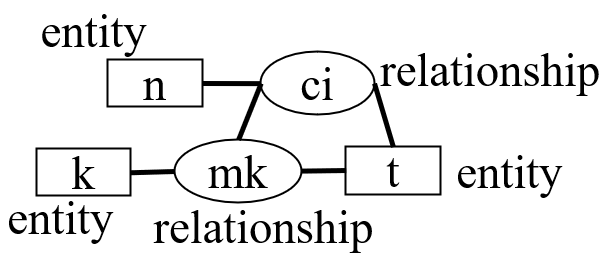
\includegraphics[width=\linewidth]{./pic/Figure6a.png}
                \end{minipage}
            }
            \subfigure[\normalsize{Sub-queries}]
            {
                \begin{minipage}[t]{0.47\linewidth}
                    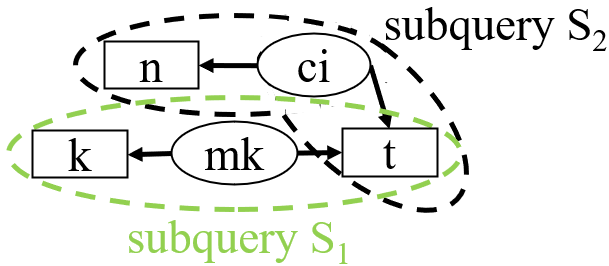
\includegraphics[width=\linewidth]{./pic/Figure6b.png}
                \end{minipage}
            }
            \centering
            \caption{Join graph split by \textit{RelationshipCenter}}
            \label{F6}
            \Description{}
        \end{figure}
        \begin{Example}[RelationshipCenter] \label{E4}
            As shown in Figure \ref{F6}(a), the query consists of one non-foreign key join ($mk \bowtie ci$) and four foreign key joins ($k \bowtie mk$, $t \bowtie mk$, $t \bowtie ci$ and $n \bowtie ci$). Hence, relation $mk$ and $ci$ are relationships and relation $k$, $n$, $t$ are entities. Then as shown in Figure \ref{F6}(b), we first remove $mk \bowtie ci$ because it is redundant, then draw a directed graph with four edges ($E_1=mk \rightarrow k$, $E_2=mk \rightarrow t$, $E_3=ci \rightarrow t$ and $E_4=ci \rightarrow n$), corresponding to join predicates. Next, consider all relations: relation $k$, $n$ and $t$ don't connect to any other relation, hence we do not create sub-queries for them; relation $mk$ connects to $k$ and $t$, resulting in sub-query $S_1=\sigma_{f_k}(k) \bowtie mk \bowtie \sigma_{f_t}(t)$; relation $ci$ connects to $n$ and $t$, and we have sub-query $S_2=\sigma_{f_n}(n) \bowtie ci \bowtie \sigma_{f_t}(t)$.
        \end{Example}\par
        Then, to illustrate that the query splitting algorithm is essential for the performance, we propose two other algorithms (\textit{MinSubquery} and \textit{EntityCenter}) for contrast and compare them with \textit{RelationshipCenter} in Section \ref{S5}.

    \subsubsection{MinSubquery} \label{S411}
        This is the most straightforward query splitting algorithm, in which we split the query into minimal sub-queries. For each select predicate that spans more than one relation, we use those relations to construct a relation set $\textbf{\textit{R}}_i$. Then we construct the set of select predicates $\textbf{\textit{S}}_i$ to contain all the select predicates over $\textbf{\textit{R}}_i$. We use an example query (shown in Figure \ref{F19}(a)) to demonstrate the procedure of \textit{MinSubquery} below.
        \begin{Example}[MinSubquery] \label{E3}
            As shown in Figure \ref{F7}(a), there are five join predicates (denoted by $k \bowtie mk$, $mk \bowtie ci$, $n \bowtie ci$, $t \bowtie mk$ and $t \bowtie ci$) and three select predicates over relation $k$, $n$, and $t$ (denoted by $f_k$, $f_n$ and $f_t$). To create sub-queries, first construct the following relation sets involved in join predicates: $\textbf{\textit{R}}_1=\{k,mk\}$, $\textbf{\textit{R}}_2=\{ci,mk\}$, $\textbf{\textit{R}}_3=\{ci,n\}$, $\textbf{\textit{R}}_4=\{mk,t\}$, $\textbf{\textit{R}}_5=\{ci,t\}$. Then, for each relation set $\textbf{\textit{R}}_i$, $\textbf{\textit{S}}_i$ is equal to the union of all select predicates in the original query over $\textbf{\textit{R}}_i$. As shown in Figure \ref{F7}(b), this results in five sub-queries $q_1=\sigma_{f_k}(k) \bowtie mk$, $q_2=mk \bowtie ci$, $q_3=\sigma_{f_n}(n) \bowtie ci$, $q_4=\sigma_{f_t}(t) \bowtie mk$ and $q_5=ci \bowtie \sigma_{f_t}(t)$.
        \end{Example}
        \begin{figure}[htb]
            \subfigure[\normalsize{The example query}]
            {
                \begin{minipage}[t]{0.47\linewidth}
                    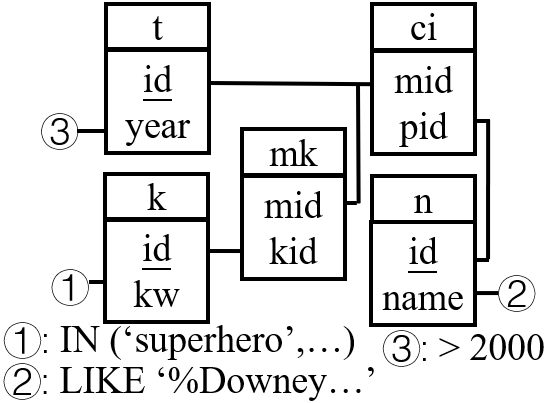
\includegraphics[width=\linewidth]{./pic/Figure7a.png}
                \end{minipage}
            }
            \subfigure[\normalsize{Sub-queries}]
            {
                \begin{minipage}[t]{0.47\linewidth}
                    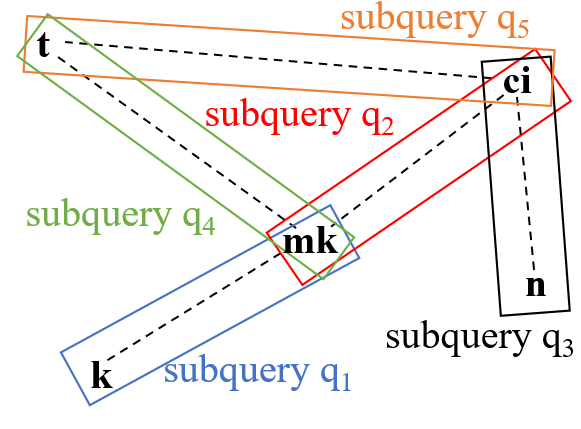
\includegraphics[width=\linewidth]{./pic/Figure7b.png}
                \end{minipage}
            }
            \centering
            \caption{Join graph split by \textit{MinSubquery}}
            \label{F7}
            \Description{}
        \end{figure}
    
    
    \subsubsection{EntityCenter} \label{S413}
        If we reverse the direction of edges in the directed graph in \textit{RelationshipCenter}, we can get another query splitting algorithm. In this algorithm, the centers of sub-queries are entity relations, and we name this algorithm \textit{EntityCenter}.
    
\subsection{Execution Order Decision} \label{S42}
    In this section, we propose some feasible criteria to decide which sub-query to execute each time. Although we have proved that execution order does not affect the correctness of \textit{query split}, different execution orders can lead to different execution time. Therefore, we give some feasible implementations as the candidates and evaluate their efficiency in Section \ref{S5}.
    \subsubsection{Heuristic-based Algorithm} \label{S421}
\textcolor{blue}{
    We propose a heuristic rule to order the sub-queries based on the \textit{ranking function}. We first take the execution plans of the sub-query as input and assign a numeric value to each by \textit{ranking function}. Then, we choose the sub-query with the lowest numeric value each time and return this sub-query and its execution plan to execute.
}\par
\textcolor{blue}{
    To build the ranking function, we need to consider what parameters we can get from a given plan and which are suitable inputs for ranking functions. For a given plan, we can get the cost estimation of that plan and its cardinality estimation. Intuitively, the cost of a plan indicates the current benefit of the plan. And the cardinality of the result represents the future benefit of the plan, since a small intermediate result will speed up the future sub-queries. Thus, we take both cost estimation and row estimation of the sub-query as candidate inputs for ranking functions.
}\par
    We have designed some ranking functions for the algorithm in Table \ref{T2}. We denote $q$ a sub-query and $plan(q)$ the execution plan made by optimizer, $plan(q).cost$ the estimated cost of $plan(q)$, and $row(q)$ the estimated size of its result. The most basic approach is to use only cost or row of sub-queries for ranking ($cost(q)$ and $row(q)$). However, these approaches fail to consider the future influence or the current benefit. Take both into consideration, we designed other three candidates $row\_hybrid(q)$, $hybrid\_sqrt(q)$ and $hybrid\_log(q)$ with detailed expression in Table \ref{T2}.
    \begin{table}[htb]
        \caption{The expression of different ranking functions}
        \label{T2}
        \begin{tabular}{c|c}
            \toprule
            ranking function  & expression                   \\
            \midrule
            $cost(q)$         & $plan(q).cost$               \\
            $row(q)$          & $row(q)$                     \\
            $row\_hybrid(q)$  & $plan(q).cost*row(q)$        \\
            $hybrid\_sqrt(q)$ & $plan(q).cost*\sqrt{row(q)}$ \\
            $hybrid\_log(q)$  & $plan(q).cost*\log(row(q))$  \\
            \bottomrule
        \end{tabular}
    \end{table}  
        
    \subsubsection{Global Plan-based Algorithm} \label{S422}
\textcolor{blue}{
    The order decision algorithms we introduce above are based on the sub-query perspective, which totally discards the global plan. In contrast, we propose an algorithm called \textit{global\_sel} that chooses which sub-query to execute according to the global plan.
}\par
    \textit{Global\_sel} starts the selection process with the global plan generated from the original query. Then, given an execution tree for the original query, we choose the deepest operator node, find the relations involved in the operator, and select the sub-query whose relation set contains those relations. If multiple sub-queries can be selected, we choose one of them by an arbitrary tie-breaking rule.
    \begin{figure}[htb]  
        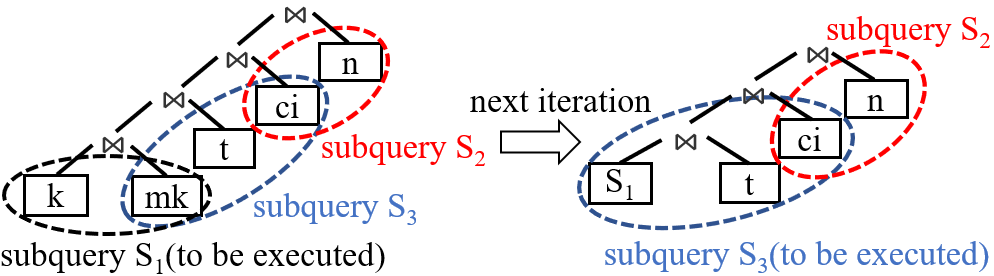
\includegraphics[width=\linewidth]{./pic/Figure8.png}
        \centering
        \caption{The illustration of \textit{global\_sel}}
        \label{F8}
        \Description{}
    \end{figure}\par
    Example \ref{E5} illustrates the procedure for the global plan-based algorithm.
    \begin{Example}[Global\_sel] \label{E5}
        We split the query into three subqueries $S_1=\sigma_{f_k}(k) \bowtie mk$, $S_2=\sigma_{f_n}(n) \bowtie ci$, and $S_3=ci \bowtie \sigma_{f_t}(t) \bowtie mk$. As shown in Figure \ref{F8}, at the beginning, the deepest non-leaf node in global plan is $k \bowtie mk$, and the involved relations are $\{k,mk\}$. Hence, sub-query $S_1$ would be first executed because it is the only sub-query whose relation set contains $k$ and $mk$. Then we materialize the sub-query result as a temporary table, and call optimizer for the remainder of the original query. In this iteration, the deepest non-leaf node in modified global plan is $S_1 \bowtie t$, so we choose $S_3$ because its relation set contains $S_1$ and $t$.
    \end{Example}